% Auto-generated by analysis/eva-bench-stats/paper_plot_perturbation.py
% Requires: graphicx, xcolor
\definecolor{pertaccent}{HTML}{00C49A}
\definecolor{pertbgnoise}{HTML}{F8E16C}
\definecolor{pertboth}{HTML}{156064}
\begin{figure}[t]
\centering
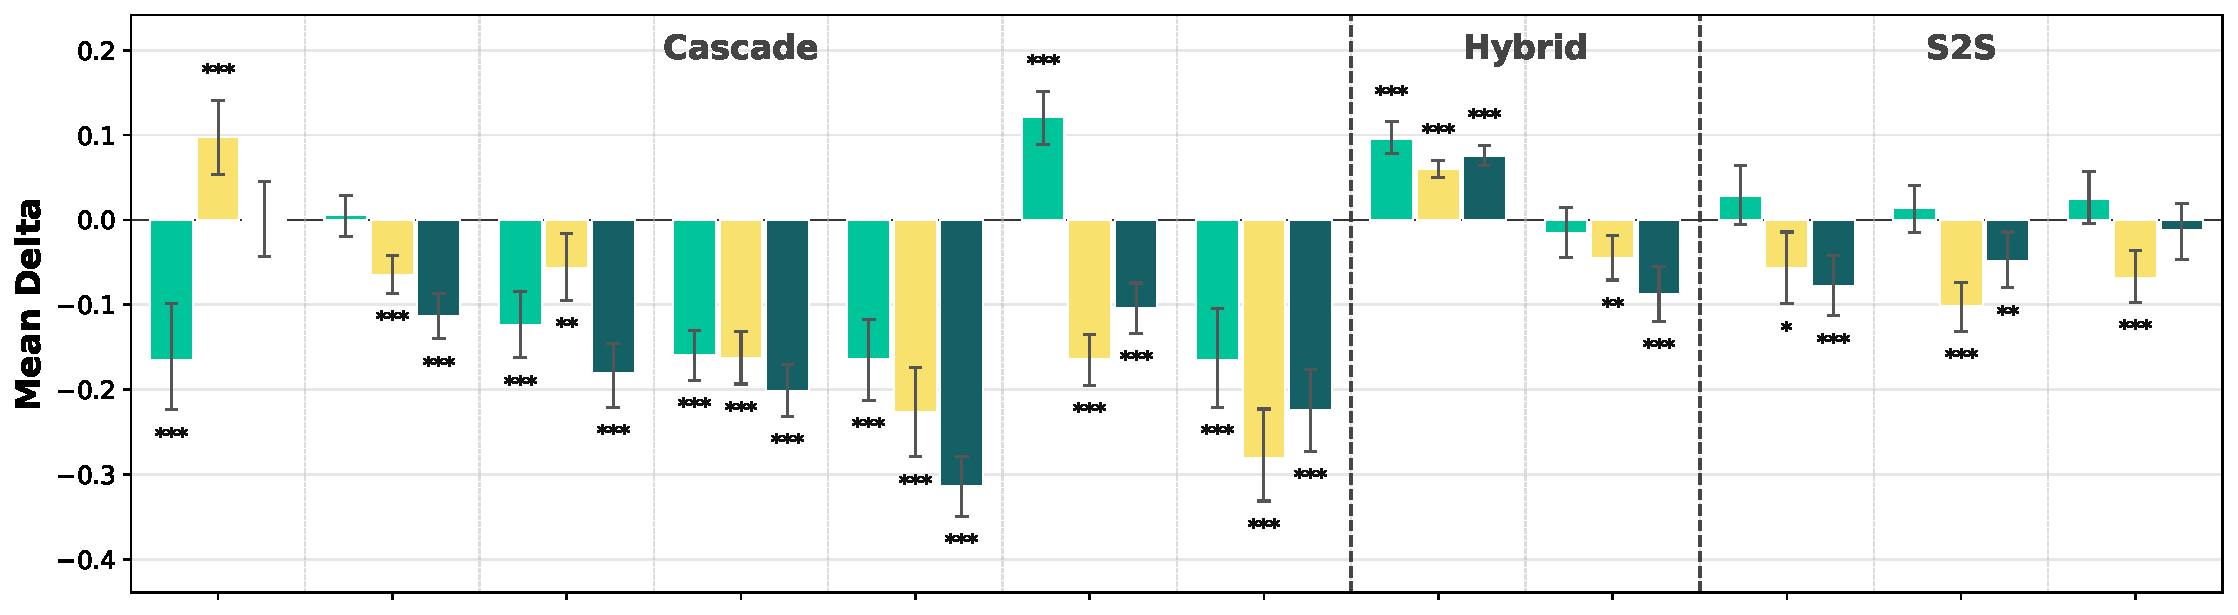
\includegraphics[width=\linewidth]{figures/perturbations/paper_turn_taking_perturbation_pooled.pdf}
\captionsetup{font=small}
\caption{Perturbation effect on  \textbf{\metricturntaking} pooled across domains. Bars show the mean delta from clean trials; 95\% bootstrap (CIs) on the per-scenario delta. Bar colors encode the perturbation condition: \textcolor{pertaccent}{$\blacksquare$}~accent, \textcolor{pertbgnoise}{$\blacksquare$}~background noise, \textcolor{pertboth}{$\blacksquare$}~accent~+~background noise. Asterisks mark cells significant after Holm-Bonferroni correction (\texttt{*}~$p<0.05$, \texttt{**}~$p<0.01$, \texttt{***}~$p<0.001$). Models listed in Appendix~\ref{app:perturbations}.}
\label{fig:perturbation-transcription-pooled-turn-taking-final}
\end{figure}
